% Created 2023-03-24 Fri 00:23
% Intended LaTeX compiler: xelatex
\documentclass[aspectratio=1610,xcolor={dvipsnames},hyperref={colorlinks,unicode,linkcolor=violet,anchorcolor=BlueViolet,citecolor=YellowOrange,filecolor=black,urlcolor=Aquamarine}]{beamer}
\usepackage{graphicx}
\usepackage{grffile}
\usepackage{longtable}
\usepackage{booktabs}
\usepackage{wrapfig}
\usepackage{rotating}
\usepackage[normalem]{ulem}
\usepackage{amsmath}
\usepackage{textcomp}
\usepackage{amssymb}
\usepackage{capt-of}
\usepackage{nicefrac}
\usepackage[dvipsnames]{xcolor}
\usepackage[colorlinks,unicode,linkcolor=violet,anchorcolor=BlueViolet,citecolor=YellowOrange,filecolor=black,urlcolor=Aquamarine]{hyperref}
\usepackage{etoolbox}
\useoutertheme{infolines}
\setbeamertemplate{frametitle}{%
\usebeamerfont{frametitle}\insertframetitle\strut%
\vskip-0\baselineskip%
\leaders\vrule width .95\paperwidth\vskip1pt%
\vskip0pt%
\nointerlineskip%
}

%% T for footer
\setbeamercolor{footlinecolor}{fg=cyan,bg=green}
\setbeamercolor{author in head/foot}{fg=blue}
\setbeamertemplate{footline}{%
\leavevmode%
\hbox{%
\begin{beamercolorbox}[wd=.26\paperwidth,ht=2.25ex,dp=1ex,left]{author in head/foot}%
\hspace*{2ex}\usebeamerfont{author in head/foot} Dept. CSE, UT Arlington
\end{beamercolorbox}%
\begin{beamercolorbox}[wd=.50\paperwidth,ht=2.25ex,dp=1ex,center]{author in head/foot}%
\usebeamerfont{title in head/foot}Scalable Modeling \& Imaging \& Learning Lab (SMILE)
\end{beamercolorbox}%
\begin{beamercolorbox}[wd=.24\paperwidth,ht=2.25ex,dp=1ex,right]{date in head/foot}%
\usebeamerfont{date in head/foot}
\insertshortdate{}\hspace*{1em}  % date
\insertframenumber/\inserttotalframenumber\hspace*{2ex}
\end{beamercolorbox}}%
\vskip0pt%
}
\setbeamerfont{footnote}{size=\tiny}
\usepackage{minted}
\usetheme{default}
\usefonttheme{serif}
\useinnertheme{circles}
\author{Nasy}
\date{Nov 18, 2022}
\title{Physics Informed Neural Networks}
\hypersetup{
 pdfauthor={Nasy},
 pdftitle={Physics Informed Neural Networks},
 pdfkeywords={},
 pdfsubject={},
 pdfcreator={Emacs 29.0.50 (Org mode 9.5.5)}, 
 pdflang={English}}
\begin{document}

\maketitle
\begin{frame}{Outline}
\tableofcontents
\end{frame}


\section{Introduction}
\label{sec:org7a0ad47}

\begin{frame}[label={sec:org8c459a7}]{Finding the inverse function of a parabola}
Given a function \(\mathcal{P}: y \rightarrow y^{2}\), where \(y \in
[0, 1]\), find a unknow function \(f\) that satisfies
\(\mathcal{P}(f(x)) = x,\ \forall x \in [0, 1]\).

\begin{columns}
\begin{column}{0.6\columnwidth}
\begin{center}
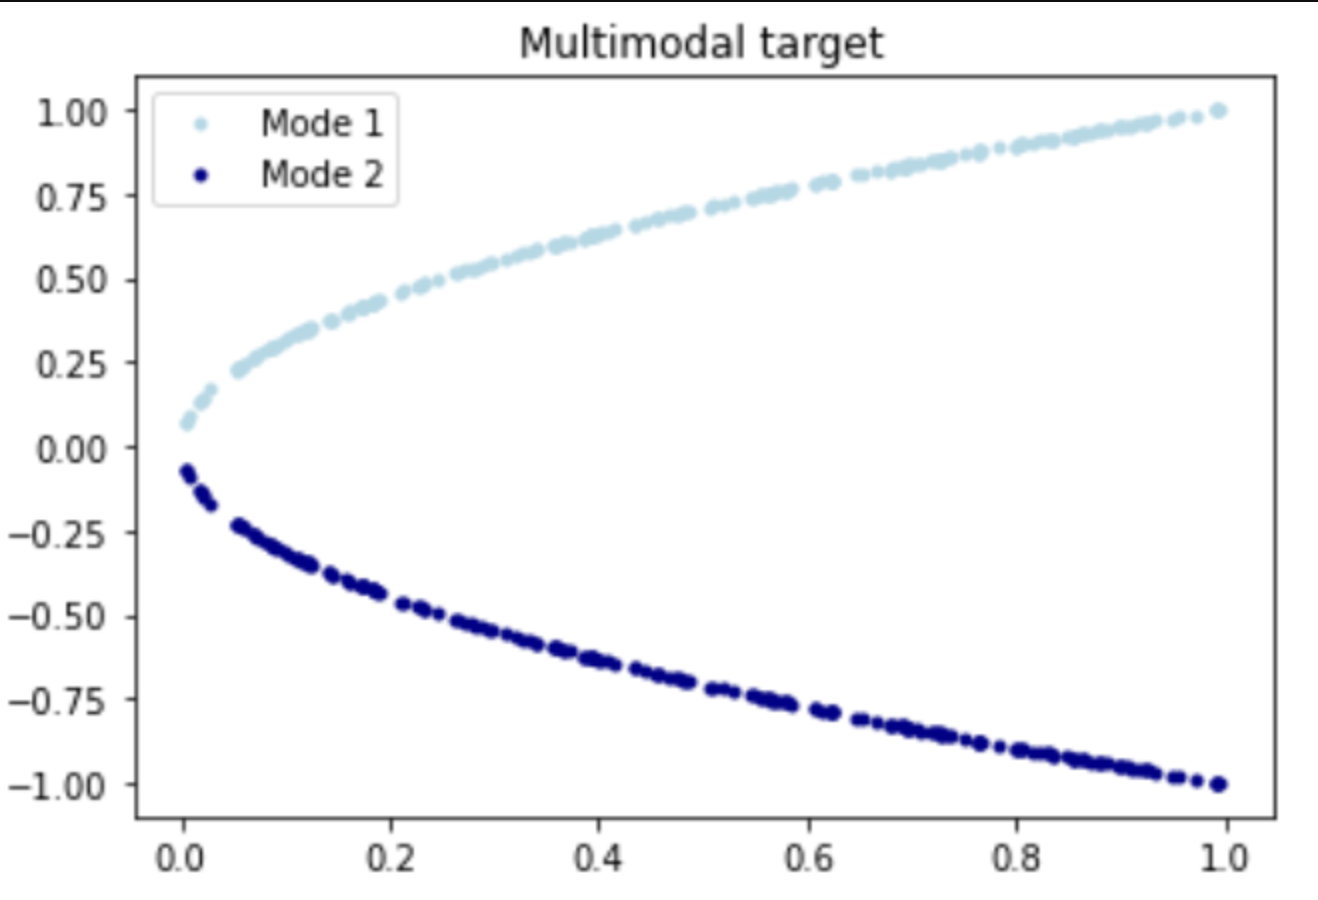
\includegraphics[width=.9\linewidth]{./p1.png}
\end{center}
\end{column}
\end{columns}
\end{frame}

\begin{frame}[label={sec:orgdd90e17}]{Classical}
\begin{columns}
\begin{column}{0.4\columnwidth}
A classical approach is to use a neural network to approximate the data points \(\Omega\):

\[f_{\theta}(x) \approx y,\ \forall (x, y) \in \Omega\]

where \(\theta\) is the parameters of the neural network.

However, nowhere near the solution.
\end{column}

\begin{column}{0.6\columnwidth}
\begin{center}
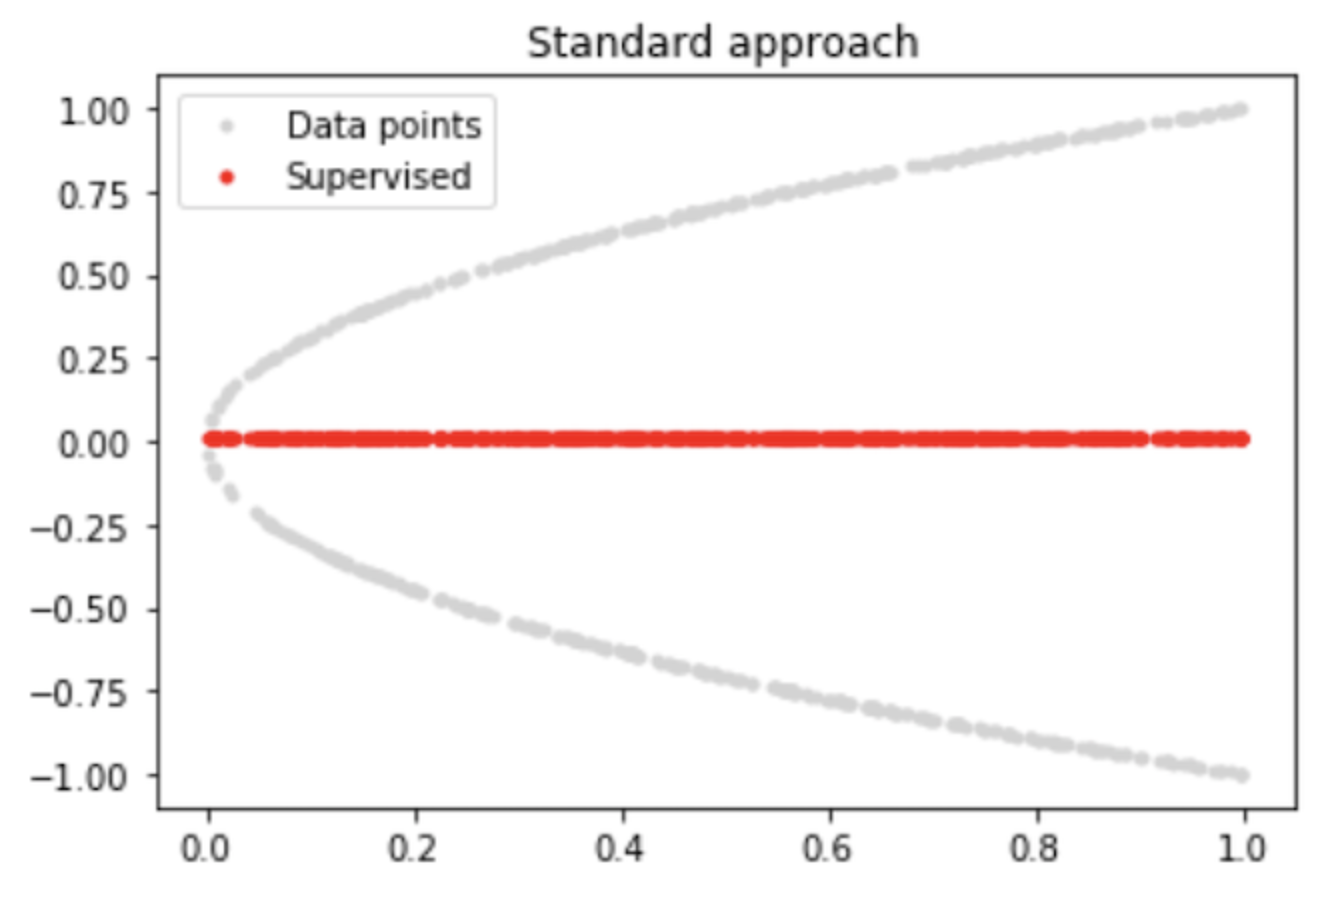
\includegraphics[width=.9\linewidth]{./p2.png}
\end{center}
\end{column}
\end{columns}
\end{frame}

\begin{frame}[label={sec:orgf972ef5}]{Physics approach}
\begin{columns}
\begin{column}{0.4\columnwidth}
\[\mathcal{P}(f_{\theta}(x)) \approx y,\ \forall (x, y) \in \Omega\]

Now, minimize the error between \(f^{2}_{\theta}(x)\)  and \(y\).
\end{column}

\begin{column}{0.6\columnwidth}
\begin{center}
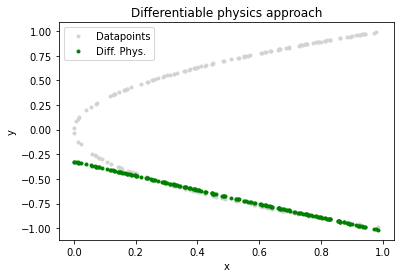
\includegraphics[width=.9\linewidth]{./p3.png}
\end{center}
\end{column}
\end{columns}
\end{frame}

\begin{frame}[label={sec:org0b84944}]{Physics Informed Neural Networks (PINNs) Definition}
Neural networks that are trained to solve supervised learning tasks
while respecting any given law of physics described by general
nonlinear partial differential equations (PDE).

\begin{center}
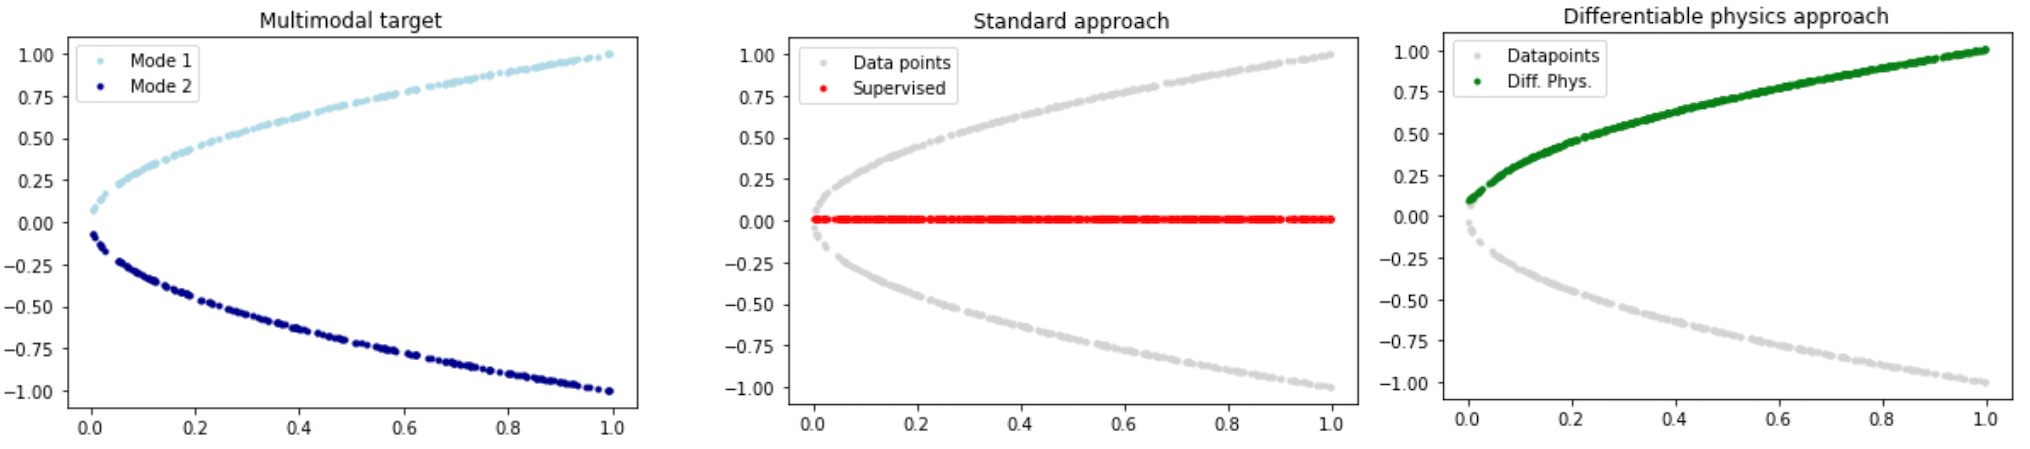
\includegraphics[width=.9\linewidth]{./p4.png}
\end{center}
\end{frame}

\section{Partial differential equations (PDE)}
\label{sec:org16c5aaf}

\subsection{Introduction}
\label{sec:orgfe3f5d8}

\begin{frame}[label={sec:org4d67a19}]{What is PDE?}
\begin{itemize}
\item Equation containing \alert{unknown functions} and \alert{its partial derivative}.
\item Describe the relationship between independent variables, unknown functions and partial derivative.
\end{itemize}

\begin{exampleblock}{Example}\label{sec:orga121ad7}
\begin{itemize}
\item \(f(x, y) = ax + by + c\), where \(a, b, c\) are unknown parameters.
\item \(u(x, y) = \alpha u(x, y) + \beta f(x, y)\) where \(u\) is the unknown function.
\item \(u_{x}(x, y) = \alpha u_{y}(x, y) + \beta f_{xy}(x, y)\) where \(u_{x}\) is the partial derivative of \(u\) with respect to \(x\), \(u_{y}\) is the partial derivative of \(u\) with respect to \(y\), and \(f_{xy}\) is the partial derivative of \(f\) with respect to \(x\) and \(y\).
\end{itemize}
\end{exampleblock}
\end{frame}

\begin{frame}[label={sec:org01d28c4}]{Notations}
\begin{itemize}
\item \(\dot{u} = \frac{\partial{u}}{\partial{t}}\)
\item \(u_{xy} = {\partial ^{2}u \over \partial y\,\partial x}\)
\item \(\nabla u (x, y, z) = u_{x} + u_{y} + u_{z}\)
\item \(\nabla \cdot \nabla u(x, y, z) = \Delta u(x,y,z) = u_{xx} + u_{yy} + u_{zz}\)
\item \(\nabla\) : nabla, or del.
\end{itemize}
\end{frame}

\subsection{PDE in the real world}
\label{sec:orga8ece5e}

\begin{frame}[label={sec:org391d88d}]{Laplace's equation}
\[\Delta \varphi = 0\]

or

\[\nabla \cdot \nabla \varphi = 0\]

or, in a 3D space:

\[\frac  {\partial ^{2}f}{\partial x^{2}}+\frac  {\partial ^{2}f}{\partial y^{2}}+\frac  {\partial ^{2}f}{\partial z^{2}} = 0\]
\end{frame}

\begin{frame}[label={sec:org4c57d1c}]{Poisson's equation}
\[\Delta \varphi = f\]

\begin{center}
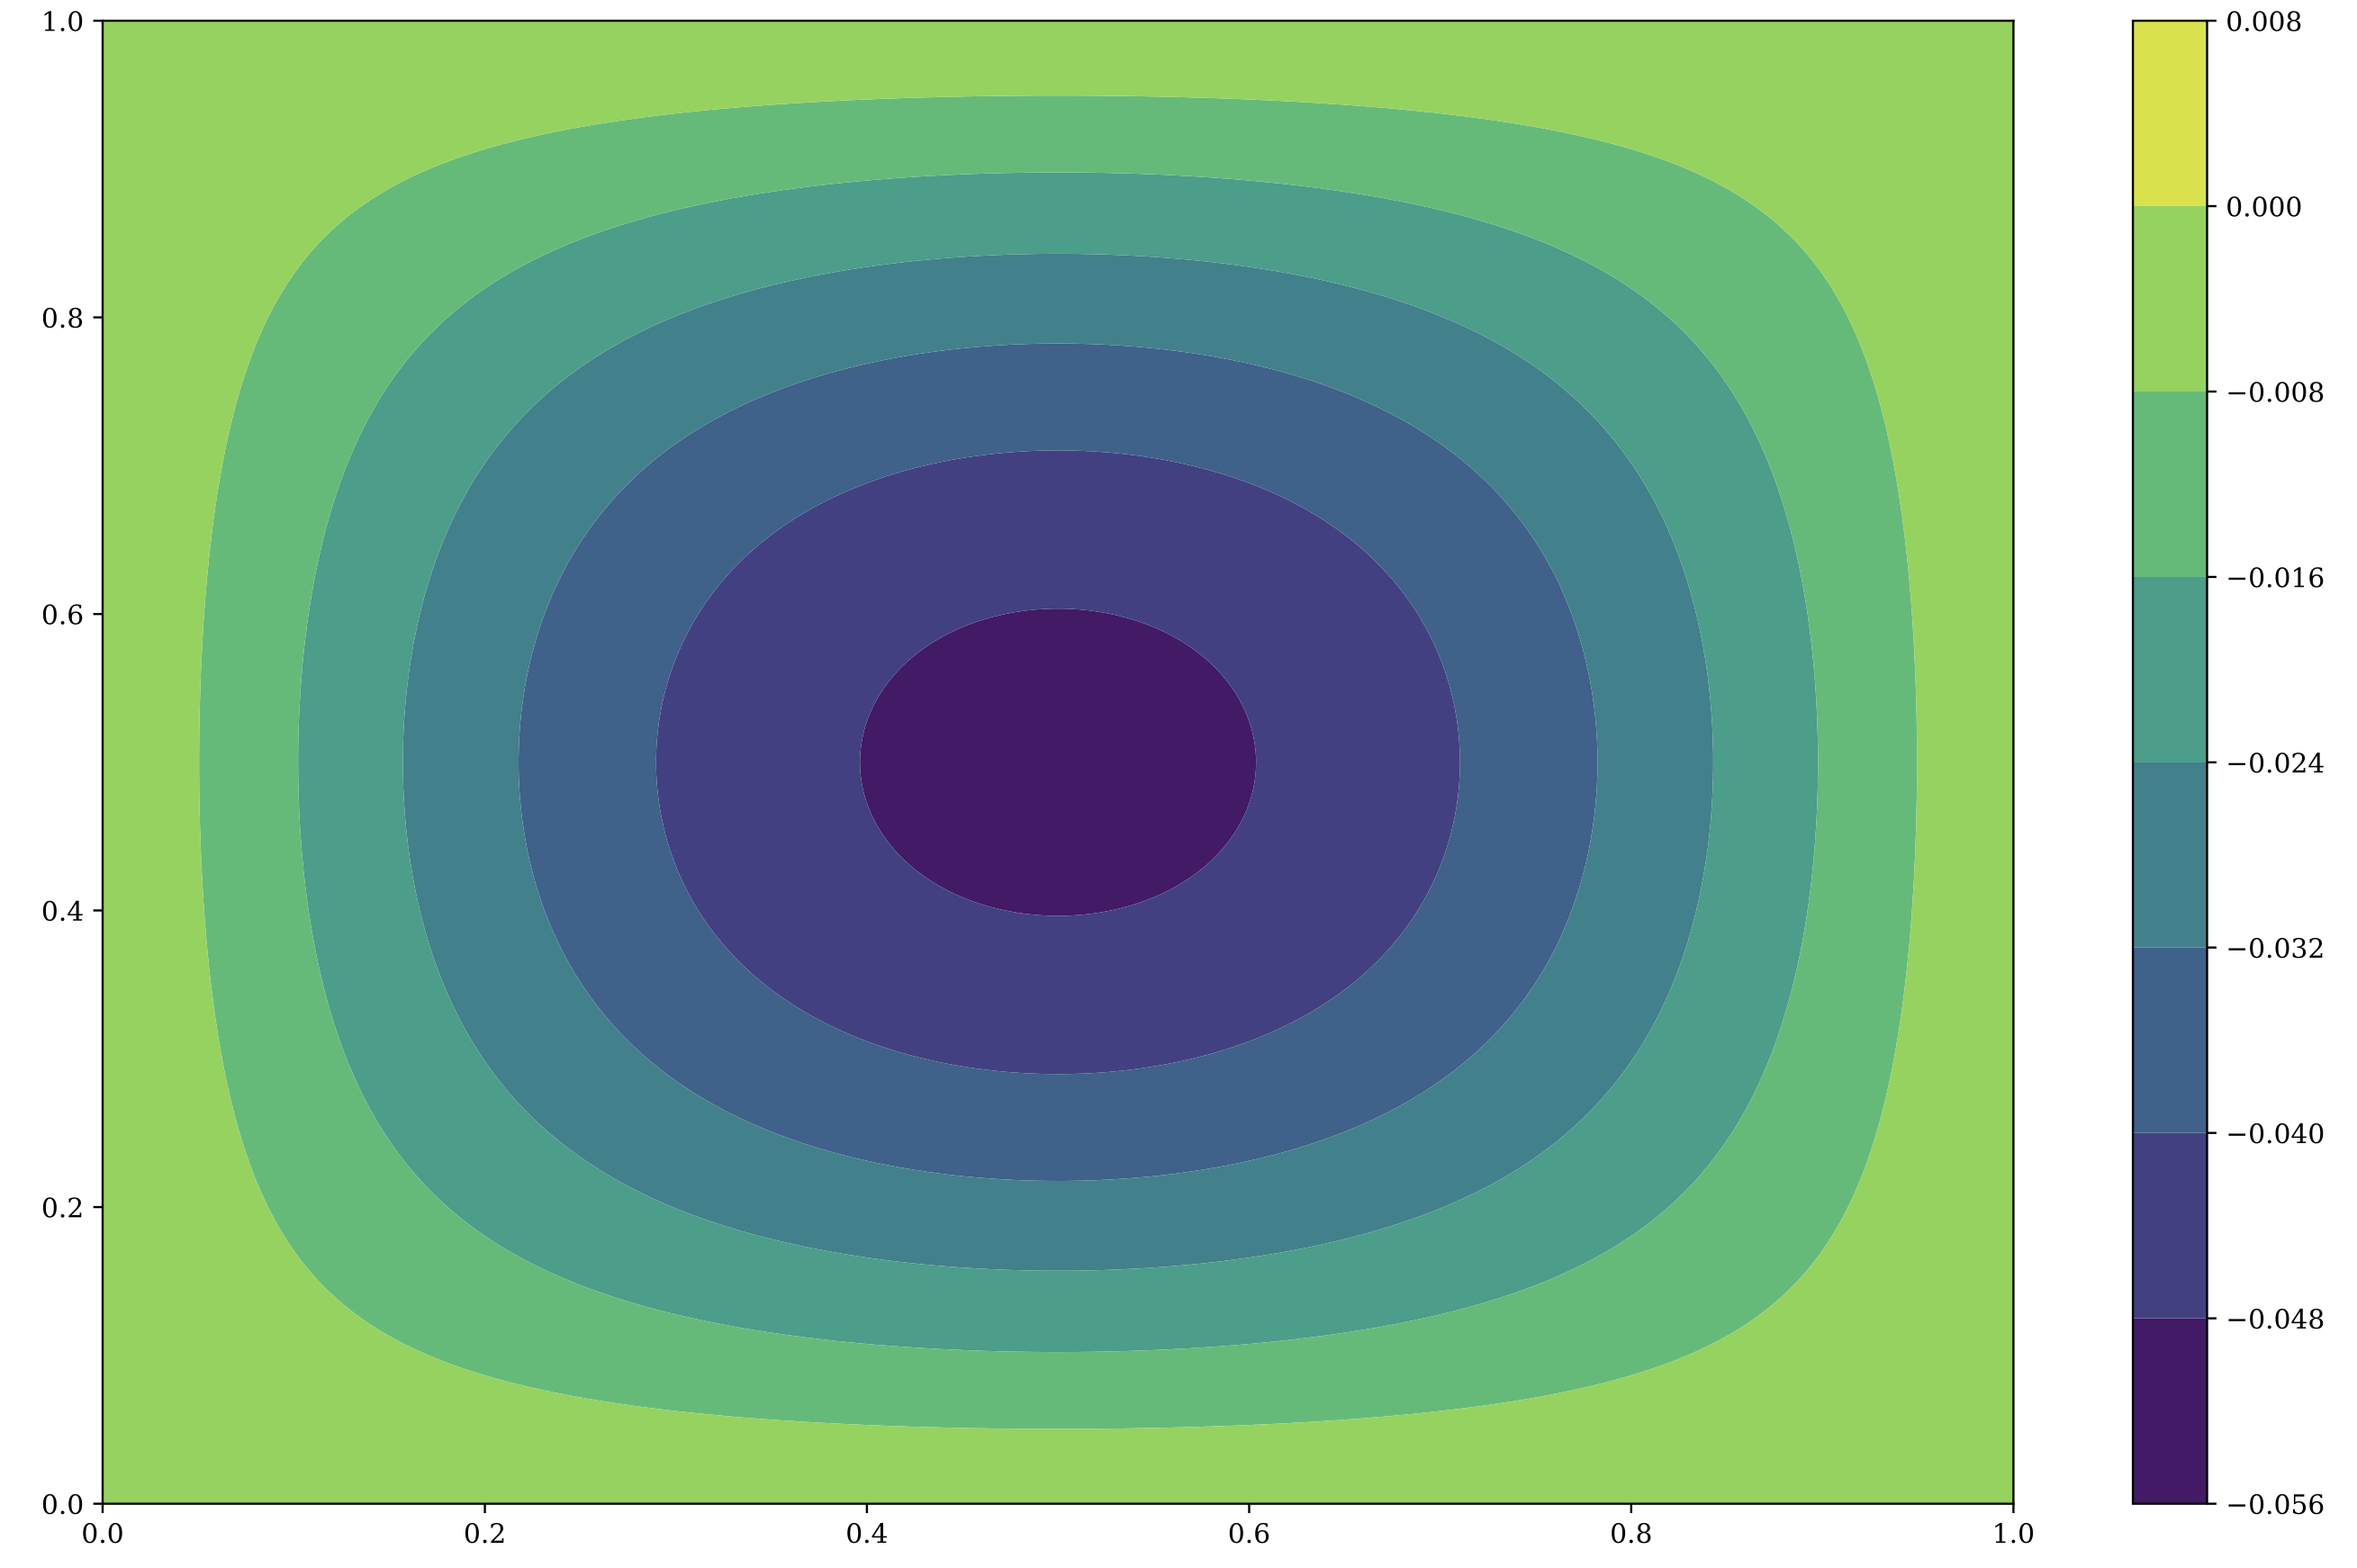
\includegraphics[height=6cm]{./p5.png}
\end{center}
\end{frame}

\begin{frame}[label={sec:orgfe4b3a3}]{Heat equation}
\[\dot{u} = \frac  {\partial u}{\partial t} = \alpha \Delta u\]

where \(\alpha\) is the thermal diffusivity.
\end{frame}

\begin{frame}[label={sec:orgb6db810}]{Wave equation}
\[\ddot {u}=c^{2}\nabla ^{2}u\]

where \(c\) is the wave speed.
\end{frame}

\begin{frame}[label={sec:org21893a0}]{Burgers' equation}
\[u_t + u u_x = \nu u_{xx}\]

\begin{description}
\item[{\(t\)}] temporal coordinate
\item[{\(x\)}] spatial coordinate
\item[{\(u(x, t)\)}] speed of fluid at the indicated spatial and temporal coordinates
\item[{\(\nu\)}] viscosity of fluid
\end{description}
\end{frame}

\subsection{Boundary conditions}
\label{sec:org242e28d}

\begin{frame}[label={sec:orgdc8fb60}]{Boundary conditions}
For a equation \(\nabla^{2}y+y=0\) in domain \(\Omega\).

\begin{itemize}
\item Dirichlet boundary condition: \(y(x)=f(x)\quad \forall x\in \partial \Omega\)
\item Neumann boundary condition: \(\frac {\partial y}{\partial \mathbf {n} }(\mathbf {x} )=f(\mathbf {x} )\quad \forall \mathbf {x} \in \partial \Omega\)
\begin{itemize}
\item Where \(f\) is a known scalar function defined on the boundary domain \(\partial \Omega\), \(\mathbf{n}\) denotes the (typically exterior) normal to the boundary.
\item The normal derivative, which shows up on the left side, is defined as \(\frac {\partial y}{\partial \mathbf {n} }(\mathbf {x} )=\nabla y(\mathbf {x} )\cdot \mathbf {\hat {n}} (\mathbf {x} )\), where \(\mathbf {\hat {n}}\) is the unit normal.
\end{itemize}
\item Robin boundary condition
\begin{itemize}
\item Combine Dirichlet and Neumann boundary conditions.
\end{itemize}
\item Periodic boundary condition
\end{itemize}
\end{frame}

\section{PINNs}
\label{sec:org493dbd1}

\begin{frame}[label={sec:org91e1858}]{Paper}
\begin{itemize}
\item Physics Informed Deep Learning (Part I): Data-driven Solutions of Nonlinear Partial Differential Equations\cite{raissiPhysicsInformedDeep2017}
\item Physics Informed Deep Learning (Part II): Data-driven Discovery of Nonlinear Partial Differential Equations\cite{raissiPhysicsInformedDeep2017a}
\end{itemize}
\end{frame}

\begin{frame}[label={sec:orgac712d9}]{Problem}
\begin{itemize}
\item Data-driven solution and data-driven discovery
\item Continuous time and discrete time models
\end{itemize}
\end{frame}

\subsection{Data-driven solution with continuous time}
\label{sec:org3c1b7dc}

\begin{frame}[label={sec:org672ff1b}]{Data-driven solution with continuous time}
General PDE Form:

\[u_t + \mathcal{N}[u] = 0,\ x \in \Omega, \ t\in[0,T]\]

where:
\begin{description}
\item[{\(\mathcal{N}[u]\)}] nonlinear differential operator
\item[{\(u(t, x)\)}] unknown function (solution).
\item[{\(\Omega\)}] spatial domain.
\item[{\(t\)}] time.
\end{description}
\end{frame}

\begin{frame}[label={sec:orgde2178e}]{Physics informed neural network}
\begin{itemize}
\item A neural network \(u_{\theta} \approx u\), where \(\theta\) is the parameters of the neural network.
\item A \alert{physics informed neural network} \(f_{\theta} = {u_{\theta}}_{t} + \mathcal{N}[u_{\theta}]\).
\item Target: \(f_{\theta} \approx u_{t} + \mathcal{N}[u]\) and \(u_{\theta} \approx u\).
\begin{itemize}
\item \(\mathcal{L} = \mathcal{L}_{f} + \mathcal{L}_{u}\)
\end{itemize}
\end{itemize}

\begin{center}
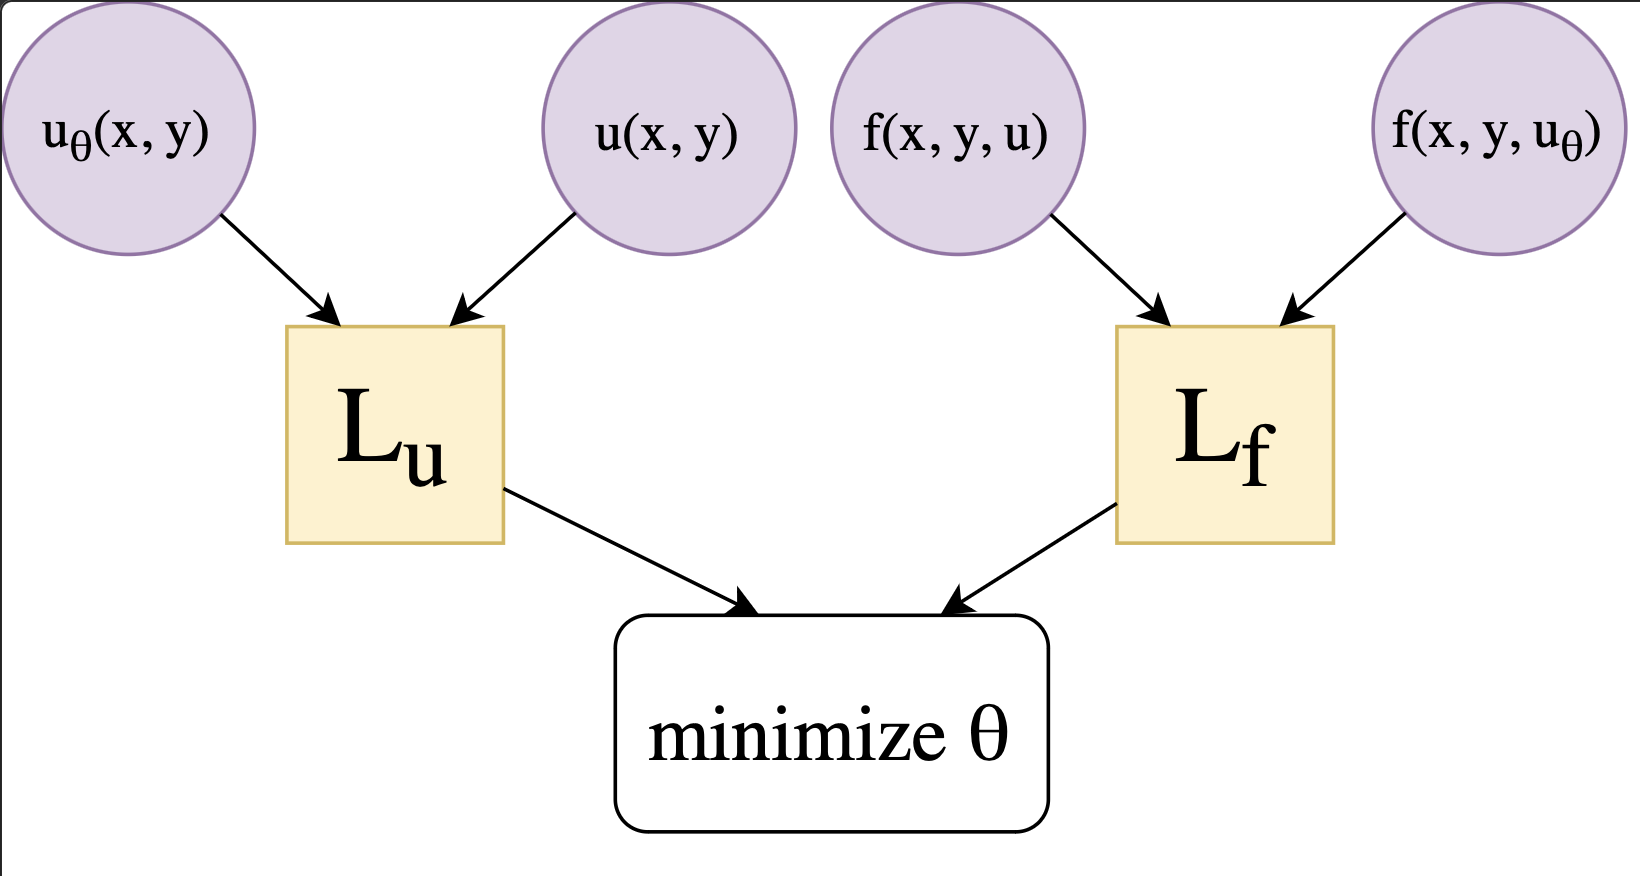
\includegraphics[height=5cm]{./p6.png}
\end{center}
\end{frame}

\begin{frame}[label={sec:org0a1c8d9}]{Example (Burgers' Equation)}
The equation:

\[u_t + u u_x = \nu u_{xx}\]

Here, already know \(\nu = 0.01 / \pi\), \(x \in [-1, 1], t \in [0, 1]\),

Thus,

\[u_{t} + uu_{x} - 0.01/\pi u_{xx} = 0 \]

And the equation along with Dirichlet boundary conditions can be written as:

\begin{itemize}
\item \(u(0, x) = -\sin(\pi x)\)
\item \(u(t, -1) = u(t, 1) = 0\)
\end{itemize}
\end{frame}

\begin{frame}[label={sec:org444c4dc}]{Target}
\begin{itemize}
\item Data:
\begin{itemize}
\item Boundary only data from boundary conditions.
\end{itemize}
\item Input: \(\{t, x\}\)
\item Output: \(u(t, x)\)
\item Target: \(f_{\theta} \approx u_{t} + \mathcal{N}[u]\) and \(u_{\theta} \approx u\).
\begin{itemize}
\item \(\mathcal{L} = \mathcal{L}_{f} + \mathcal{L}_{u}\)
\end{itemize}
\end{itemize}
\end{frame}

\begin{frame}[label={sec:org1d3afdf},fragile,containsverbatim]{Example (Burgers' Equation) with codes}
 \begin{minted}[]{python}
def u_theta(theta, t, x):
    # u_theta.apply(theta, t, x) to approx u(x, t)
    return net(theta, t, x)

def f_theta(theta, t, x):
    # See the auto diff cookbook
    # https://jax.readthedocs.io/en/latest/notebooks/autodiff_cookbook.html
    u = u_theta.apply
    u_t = jax.jacrev(u, argnums=1)(theta, t, x)
    u_x = jax.jacrev(u, argnums=2)(theta, t, x)
    u_xx = jax.hessian(u, argnums=2)(theta, t, x)
    # or jax.jacfwd(jax.jacrev(u, argnums=2), argnums=2)
    f = lambda: u_t + u * u_x - 0.01 * u_xx
    return f
\end{minted}
\end{frame}

\begin{frame}[label={sec:orgd2c9a64}]{Train and Results}
\begin{itemize}
\item Train with MLPs with L-BFGS solver (quasi-newton method).
\item Cannot use ReLU but tanh, because when we do the second order derivative, the ReLU will be 0.
\end{itemize}

\begin{center}
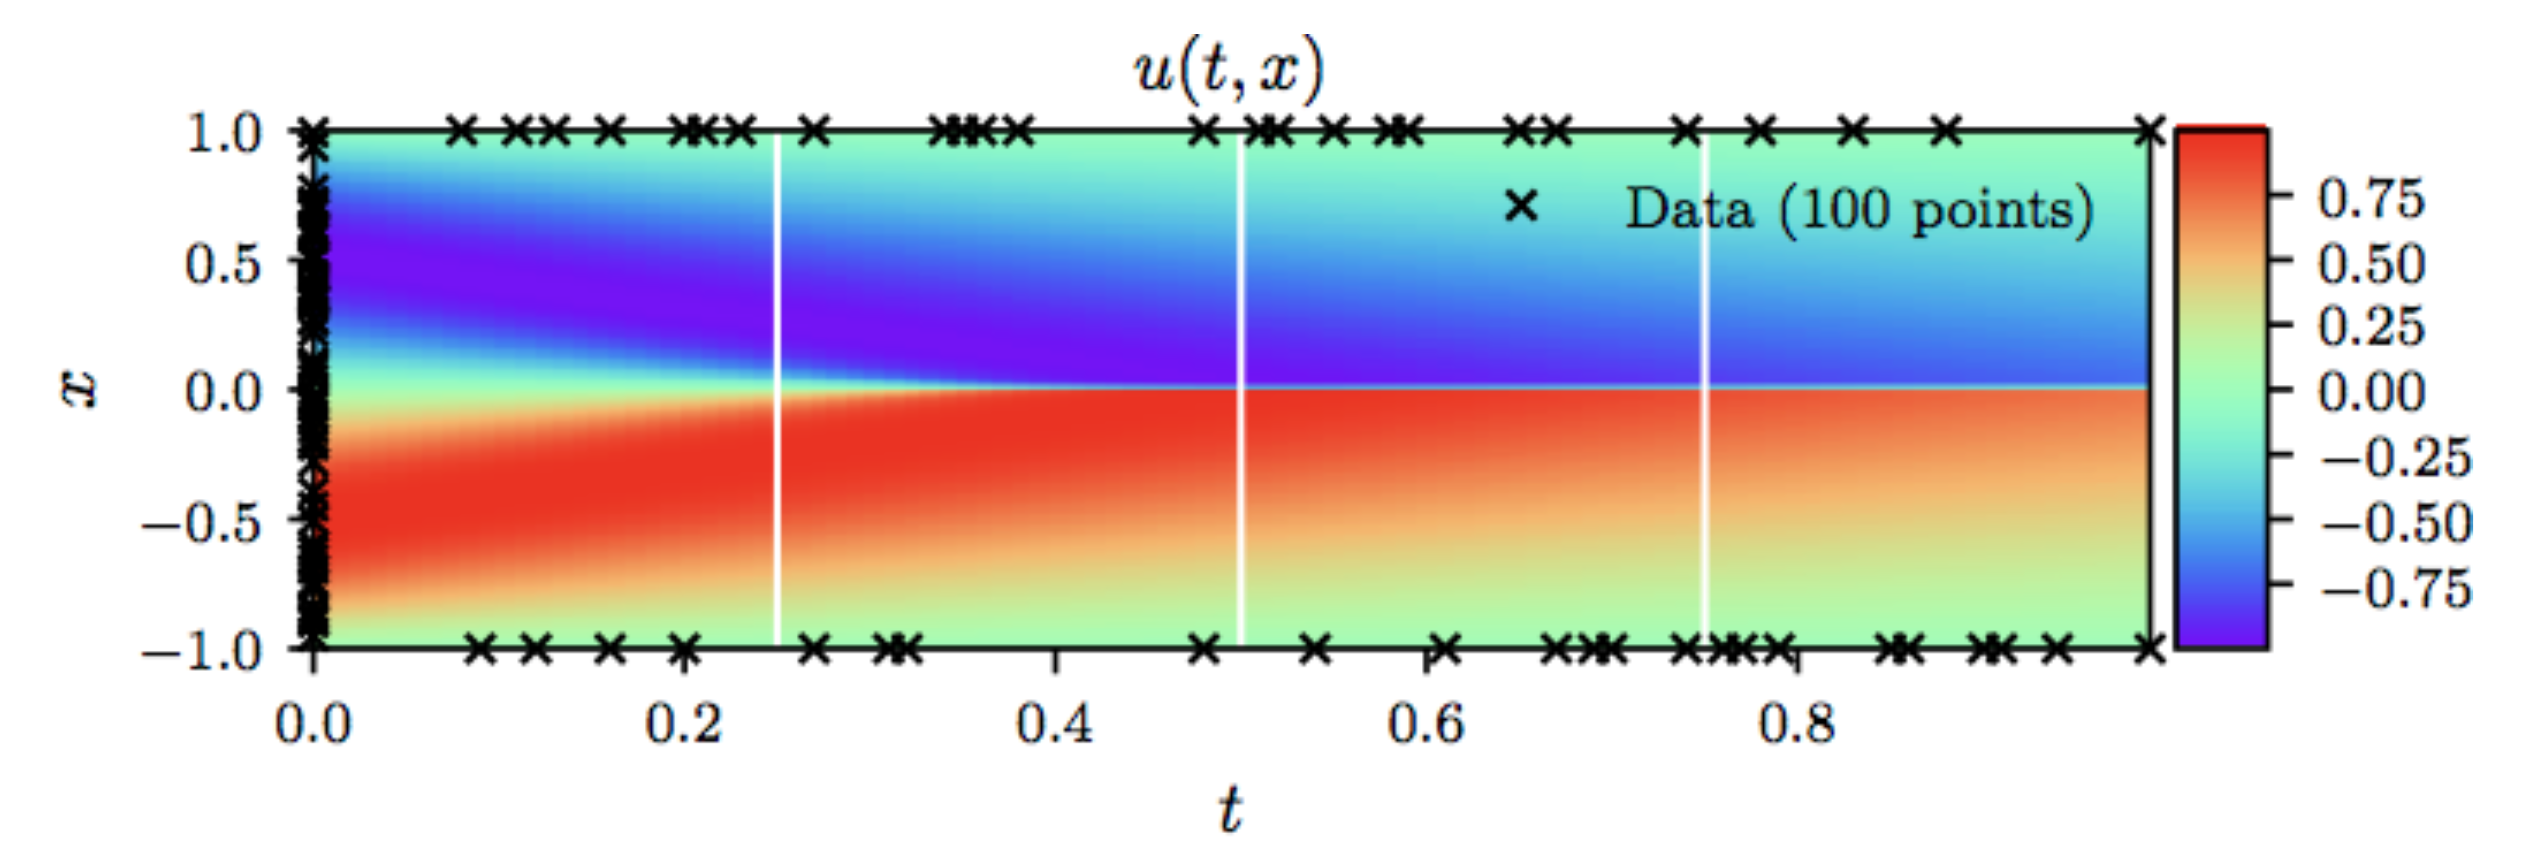
\includegraphics[width=.9\linewidth]{./p7.png}
\end{center}
\end{frame}

\subsection{Data-driven discovery with continuous time}
\label{sec:org9698a8a}

\begin{frame}[label={sec:org7b92568}]{Data-driven discovery with continuous time}
General PDE Form:

\[u_t + \mathcal{N}[u;\lambda] = 0,\ x \in \Omega, \ t\in[0,T]\]

where:
\begin{description}
\item[{\(\mathcal{N}[u;\lambda]\)}] nonlinear differential operator with parameters \(\lambda\).
\item[{\(u(t, x)\)}] unknown function (solution).
\item[{\(\Omega\)}] spatial domain.
\item[{\(t\)}] time.
\end{description}
\end{frame}

\begin{frame}[allowframebreaks]{Example (Incompressible Navier-Stokes Equation (convection–diffusion equations))}
The equations:

\[u_t + \lambda_1 (u u_x + v u_y) = -p_x + \lambda_2(u_{xx} + u_{yy}),\]
\[v_t + \lambda_1 (u v_x + v v_y) = -p_y + \lambda_2(v_{xx} + v_{yy})\],

where:
\begin{description}
\item[{\(u(t, x, y)\)}] \(x\)-component of the velocity field,
\item[{\(v(t, x, y)\)}] \(y\)-component of the velocity field,
\item[{\(p(t, x, y)\)}] pressure,
\item[{\(\lambda\)}] the unknown parameters.
\end{description}

Additional physical constraints:

\begin{itemize}
\item Solutions to the Navier-Stokes equations are searched in the set of divergence-free functions, i.e.:
\begin{itemize}
\item \(u_{x} + u_{y} = 0\)
\item which describes the conservation of mass of the fluid
\end{itemize}
\item \(u\) and \(v\) can written as a latent function \(\psi(t, x, y)\) with an assumption:
\begin{itemize}
\item \(u = \psi_{y}, v = -\psi_{x}\)
\end{itemize}
\end{itemize}
\end{frame}

\begin{frame}[label={sec:org5ffd44c}]{NS Equation figure}
\begin{center}
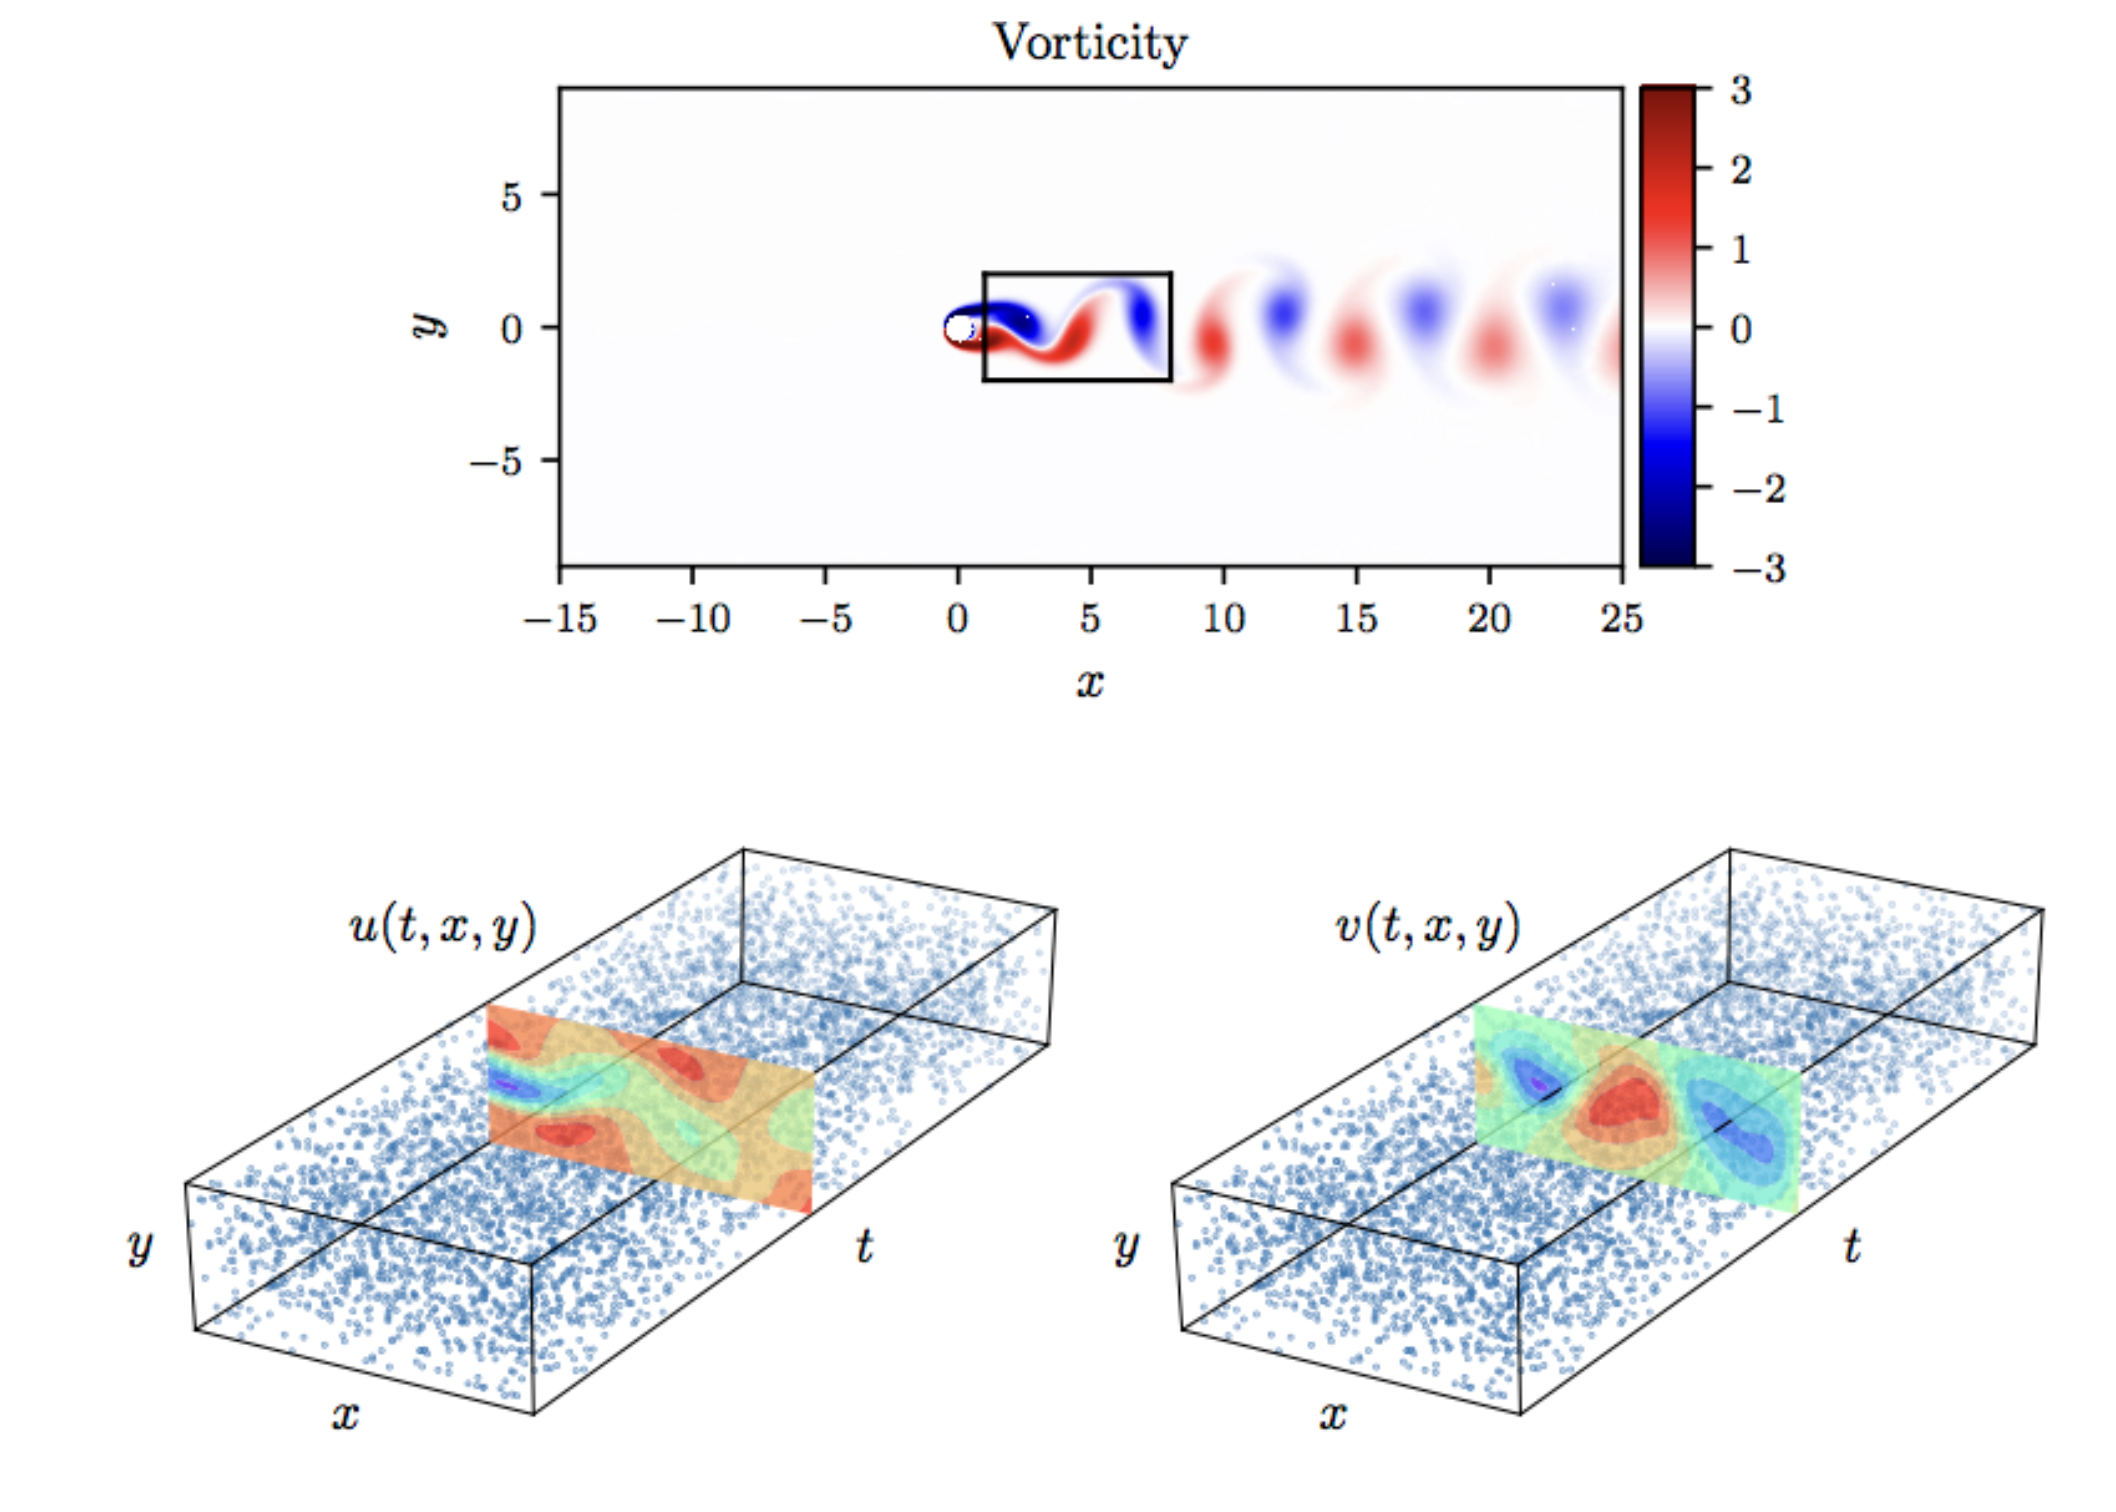
\includegraphics[height=7cm]{./p8.png}
\end{center}
\end{frame}

\begin{frame}[label={sec:org5b07541}]{Example (Navier-Stokes Equation) -- Target}
\begin{itemize}
\item The neural network equations:
\begin{itemize}
\item \(f := u_t + \lambda_1 (u u_x + v u_y) + p_x - \lambda_2(u_{xx} + u_{yy}),\)
\item \(g := v_t + \lambda_1 (u v_x + v v_y) + p_y - \lambda_2(v_{xx} + v_{yy})\)
\end{itemize}
\item Inptu: \(\{t,x,y,u,v\}\) with noisy.
\item Output: \((\psi(t, x, y), p(t, x, y))\).
\item Target:
\begin{itemize}
\item \(f_{\theta} \approx f\)
\item \(g_{\theta} \approx g\)
\item \(u_{\theta} \approx u\)
\item \(v_{\theta} \approx v\)
\end{itemize}
\end{itemize}
\end{frame}

\begin{frame}[label={sec:org5c27c39}]{Results}
\begin{center}
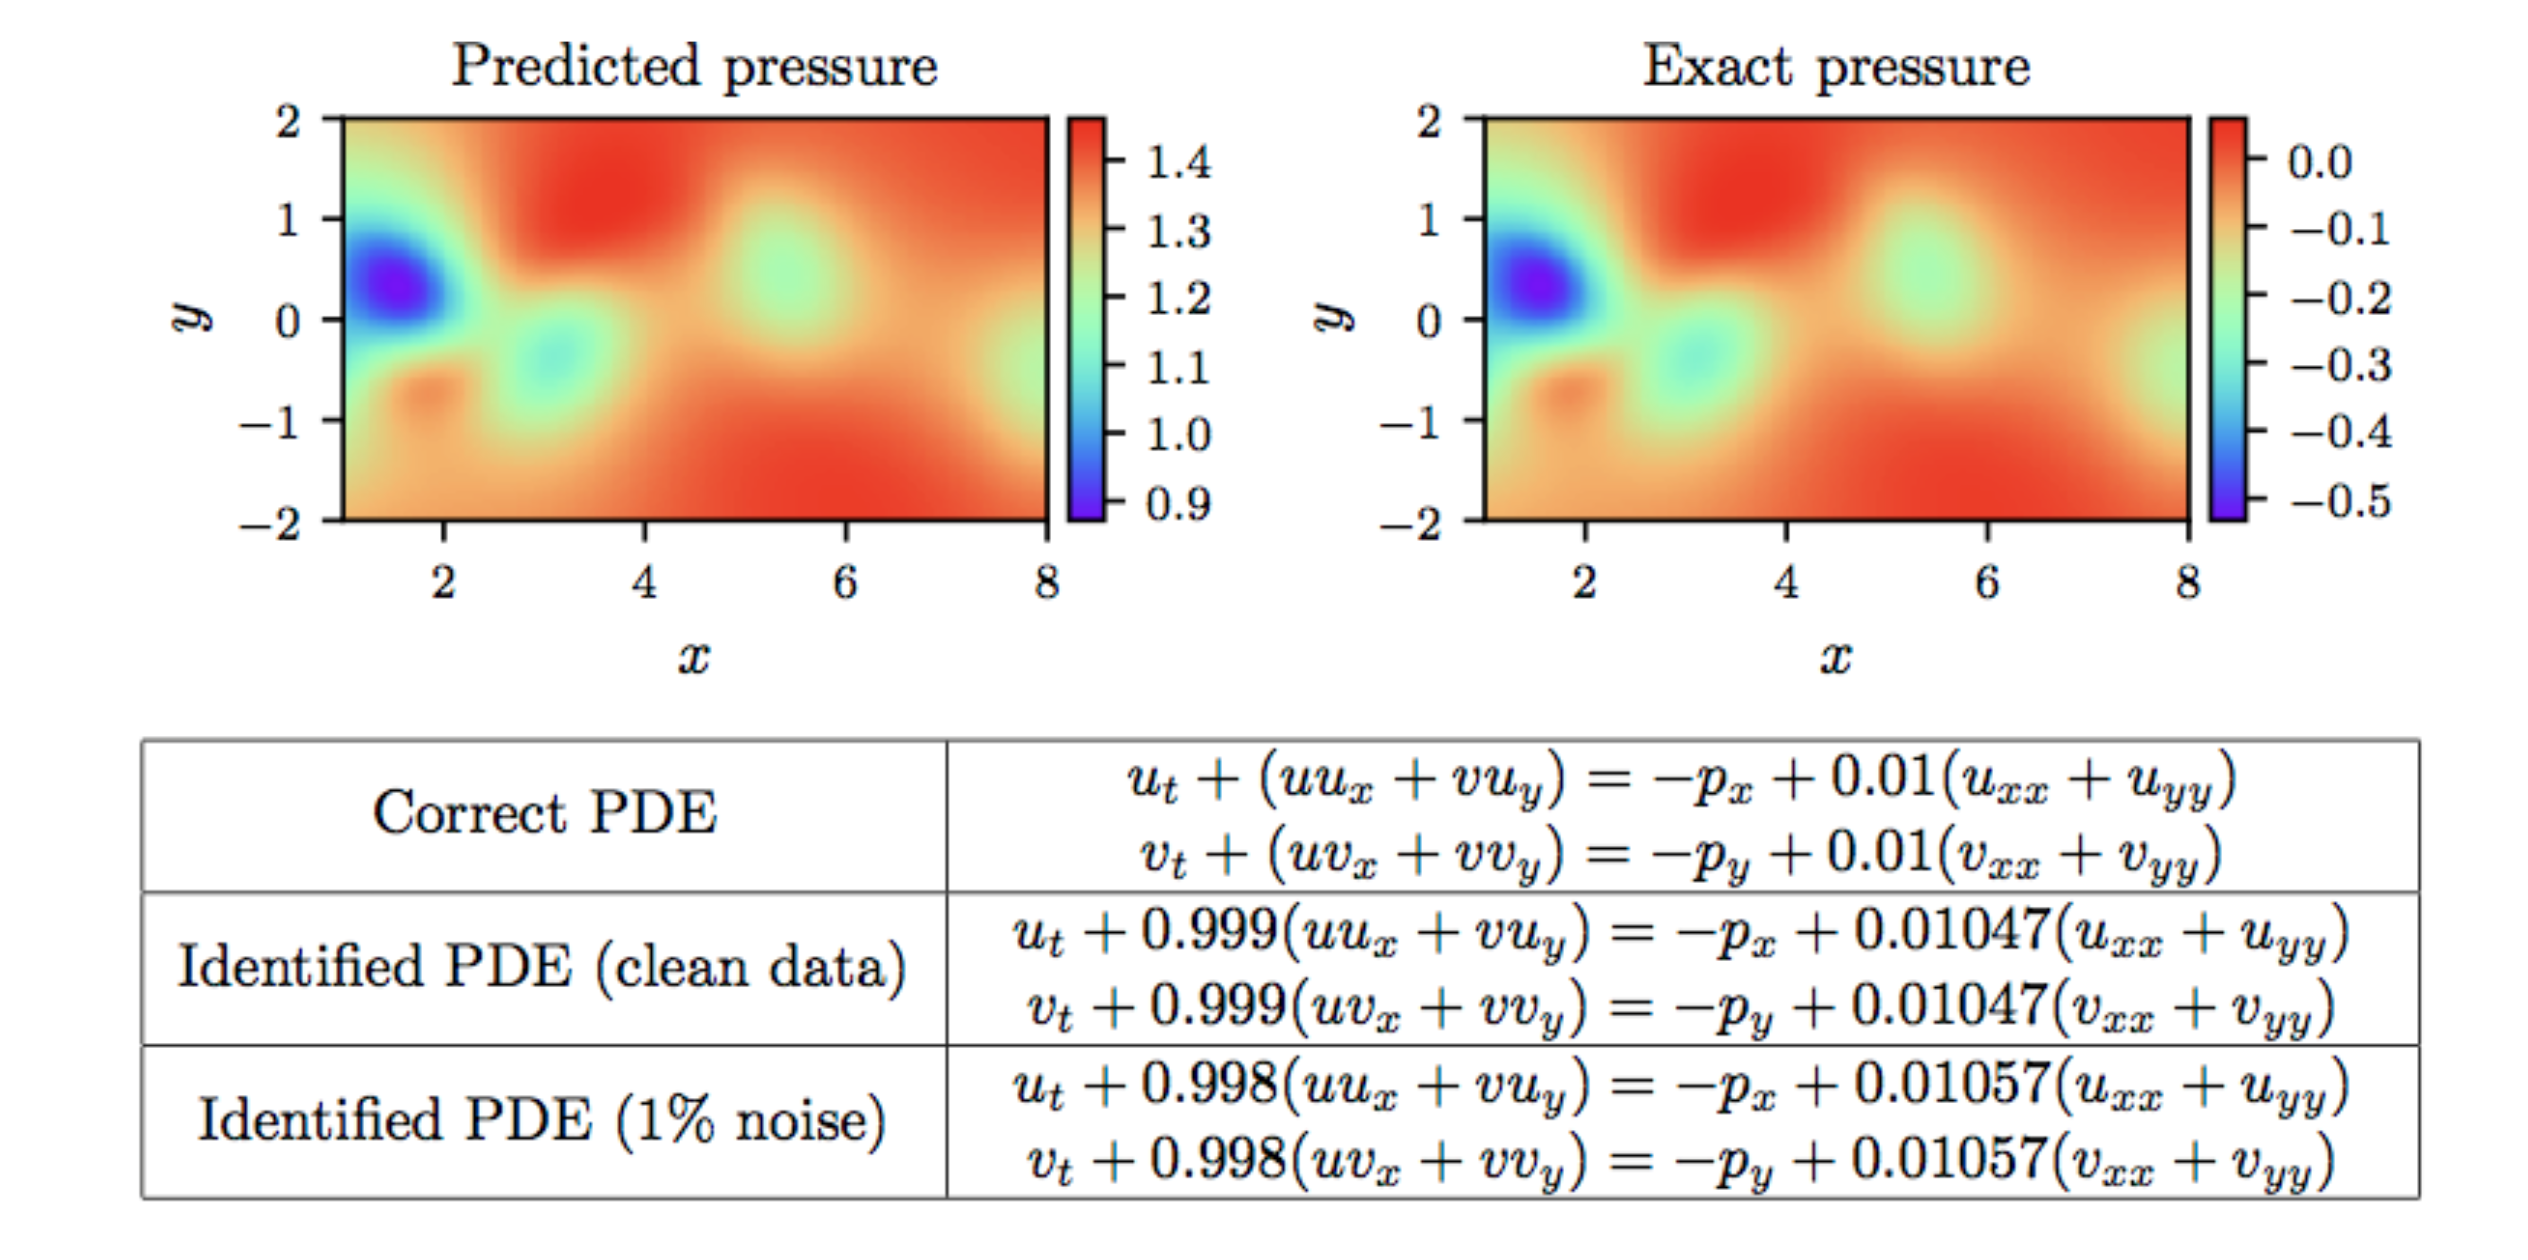
\includegraphics[width=.9\linewidth]{./p9.png}
\end{center}
\end{frame}

\section{JAX}
\label{sec:org207db80}

\begin{frame}[label={sec:org08699cc}]{Introduction}
JAX is Autograd and XLA, brought together for high-performance
numerical computing and machine learning research. It provides
composable transformations of Python+NumPy programs: differentiate,
vectorize, parallelize, Just-In-Time compile to GPU/TPU, and more.
\end{frame}

\begin{frame}[label={sec:orgb43aadd},fragile]{Pure functional}
 \begin{itemize}
\item \(f(x) = y\), always.
\item non-pure function:
\begin{itemize}
\item IO operator: \texttt{print}
\item No seed random function
\item \texttt{time}
\item Runtime error.
\end{itemize}
\end{itemize}
\end{frame}

\begin{frame}[label={sec:orgcbd9332},fragile]{Ecosystem}
 \begin{itemize}
\item JAX (jax, jaxlib)
\begin{itemize}
\item \texttt{jax}
\item \texttt{jax.numpy}
\end{itemize}
\item Haiku (dm-haiku) from deepmind
\begin{itemize}
\item Modules
\end{itemize}
\item Optax (optax) from deepmind
\begin{itemize}
\item Light
\item Linear system optimizers (\(Ax = b\))
\end{itemize}
\item JAXopt (jaxopt)
\begin{itemize}
\item Other optimizers.
\end{itemize}
\item Jraph (jraph)
\begin{itemize}
\item Standardized data structures for graphs.
\end{itemize}
\item JAX, M.D. (jax-md)
\begin{itemize}
\item JAX and Molecular Dynamics
\end{itemize}
\item RLax (rlax), and Coax (coax)
\begin{itemize}
\item Reinforcement Learning
\end{itemize}
\end{itemize}
\end{frame}

\begin{frame}[label={sec:org7b2516c},fragile,containsverbatim]{Example (def)}
 \begin{minted}[]{python}
import jax
import jax.numpy as jnp
import haiku as hk

def _u(t, x):
    return hk.MLP(jnp.concatenate([t, x], axis=-1), [10, 10, 1])

u = hk.transform_with_state(_u)
\end{minted}
\end{frame}

\begin{frame}[label={sec:org787ce60},fragile,containsverbatim]{Example (init)}
 \begin{minted}[]{python}
fake_t = jnp.ones([batch, size])
fake_x = jnp.ones([batch, size])

# theta: params
# state: training state
# rng:   random number generator
params, state = u.init(rng, fake_t, fake_x)

hk.experimental.tabulate(u)(fake_t, fake_x)
\end{minted}
\end{frame}

\begin{frame}[label={sec:org536c290},fragile,containsverbatim]{Example (loss)}
 \begin{minted}[]{python}
def loss_fn(config, ...):

    def _loss(params, t, x):
        u_theta = u.apply(params, t, x)
        ...
        loss = _f
        return loss

    return _loss

loss = loss_fn(config, ...)
\end{minted}
\end{frame}

\begin{frame}[label={sec:orgfadc2c6},fragile,containsverbatim]{Example (optim)}
 \begin{minted}[]{python}
import optax

lr = optax.linear_schedule(
    0.001,       # init
    0.001 / 10,  # final
    1,           # steps change to final
    150          # start linear decay after steps
)

opt = optax.adam(learning_rate=lr)
opt = optax.adamax(learning_rate=lr)
\end{minted}
\end{frame}

\begin{frame}[label={sec:org6984ed2},fragile,containsverbatim]{Example (solver)}
 \begin{minted}[]{python}
import jaxopt

# Linear solver
solver = jaxopt.OptaxSolver(
    loss,
    opt,
    maxiter=epochs,
    ...
)

# non-linear solver
solver = jaxopt.LBFGS(
    loss,
    maxiter=epochs,
    ...
)

opt_state = solver.init(params, state)
update = solver.update
\end{minted}
\end{frame}

\begin{frame}[label={sec:org86d3bb6},fragile]{Example (train)}
 \begin{minted}[]{python}
# init
params, state, opt_state, update


for batch in data:
    params, state = update(params, state, batch)
\end{minted}
\end{frame}

\begin{frame}[label={sec:org3084c38},fragile]{Example (parallel)}
 \begin{minted}[]{python}
# Use pjit
from jax.experimental.maps import Mesh, ResourceEnv, thread_resources
from jax.experimental.pjit import PartitionSpec, pjit

mesh = Mesh(np.asarray(jax.devices(), dtype=object), ["data", ...])
thread_resources.env = ResourceEnv(physical_mesh=mesh, loops=())

update = pjit(
    solver.update,
    in_axis_resources=[
        None,  # params
        None,  # state
        PartitionSpec("data"),  # batch
    ],
    out_axis_resources=None,
)
\end{minted}
\end{frame}

\section{Conclusion}
\label{sec:org21faefe}

\begin{frame}[label={sec:orgb0d717a}]{Conclusion}
\begin{itemize}
\item Find an inverse function of a parabola
\begin{itemize}
\item Classical
\item Physics informed
\end{itemize}
\item PDE
\begin{itemize}
\item PDE example
\item PDE boundary
\end{itemize}
\item PINNs
\begin{itemize}
\item Data-driven solution with continuous time
\begin{itemize}
\item Burgers' equation
\end{itemize}
\item Data-driven discovery with continuous time
\begin{itemize}
\item Navier-Stokes equation
\end{itemize}
\end{itemize}
\end{itemize}
\end{frame}

\section{Refs}
\label{sec:org93842f9}

\begin{frame}[allowframebreaks]{Refs}
\bibliographystyle{oscola}
\bibliography{~/.emacs.d/萚兮/時/refs/ref}
\end{frame}
\end{document}